%%%%%%%%%%%%%%%%%%%%%%%%%%%%%%%%%%%%%%%%%
% Beamer Presentation
% LaTeX Template
% Version 1.0 (10/11/12)
%
% This template has been downloaded from:
% http://www.LaTeXTemplates.com
%
% License:
% CC BY-NC-SA 3.0 (http://creativecommons.org/licenses/by-nc-sa/3.0/)
%
%%%%%%%%%%%%%%%%%%%%%%%%%%%%%%%%%%%%%%%%%

%----------------------------------------------------------------------------------------
%	PACKAGES AND THEMES
%----------------------------------------------------------------------------------------

\documentclass{beamer}

\mode<presentation> {

% The Beamer class comes with a number of default slide themes
% which change the colors and layouts of slides. Below this is a list
% of all the themes, uncomment each in turn to see what they look like.

%\usetheme{default}
%\usetheme{AnnArbor} %no
%\usetheme{Antibes}
%\usetheme{Bergen} %no
%\usetheme{Berkeley} %no
%\usetheme{Berlin}
%\usetheme{Boadilla}
%\usetheme{CambridgeUS}
%\usetheme{Copenhagen}
\usetheme{Darmstadt}
%\usetheme{Dresden}
%\usetheme{Frankfurt}
%\usetheme{Goettingen}
%\usetheme{Hannover}
%\usetheme{Ilmenau}
%\usetheme{JuanLesPins}
%\usetheme{Luebeck}
%\usetheme{Madrid}
%\usetheme{Malmoe}
%\usetheme{Marburg}
%\usetheme{Montpellier}
%\usetheme{PaloAlto}
%\usetheme{Pittsburgh}
%\usetheme{Rochester}
%\usetheme{Singapore}
%\usetheme{Szeged}
%\usetheme{Warsaw}

% As well as themes, the Beamer class has a number of color themes
% for any slide theme. Uncomment each of these in turn to see how it
% changes the colors of your current slide theme.

%\usecolortheme{albatross}
\usecolortheme{beaver}
%\usecolortheme{beetle}
%\usecolortheme{crane}
%\usecolortheme{dolphin}
%\usecolortheme{dove}
%\usecolortheme{fly}
%\usecolortheme{lily}
%\usecolortheme{orchid}
%\usecolortheme{rose}
%\usecolortheme{seagull}
%\usecolortheme{seahorse}
%\usecolortheme{whale}
%\usecolortheme{wolverine}

%\setbeamertemplate{footline} % To remove the footer line in all slides uncomment this line
%\setbeamertemplate{footline}[page number] % To replace the footer line in all slides with a simple slide count uncomment this line

%\setbeamertemplate{navigation symbols}{} % To remove the navigation symbols from the bottom of all slides uncomment this line
}

\usepackage{graphicx} % Allows including images
\usepackage{booktabs} % Allows the use of \toprule, \midrule and \bottomrule in tables

\DeclareMathOperator{\Ad}{Ad}
\DeclareMathOperator{\ad}{ad}
\DeclareMathOperator{\id}{id}
\DeclareMathOperator{\codim}{codim}

%----------------------------------------------------------------------------------------
%	TITLE PAGE
%----------------------------------------------------------------------------------------

\title[Localization]{Equivariant Cohomology and Localization} % The short title appears at the bottom of every slide, the full title is only on the title page

\author{Nelvis Fornasin} % Your name
\institute[LMU] % Your institution as it will appear on the bottom of every slide, may be shorthand to save space
{
Ludwig-Maximilians-Universit\"at M\"unchen  \\ % Your institution for the title page
\medskip
%\textit{john@smith.com} % Your email address
}
\date{8 June, 2016} % Date, can be changed to a custom date

\begin{document}

\begin{frame}
\titlepage % Print the title page as the first slide
\end{frame}

\begin{frame}
\frametitle{Overview} % Table of contents slide, comment this block out to remove it
\tableofcontents % Throughout your presentation, if you choose to use \section{} and \subsection{} commands, these will automatically be printed on this slide as an overview of your presentation
\end{frame}

%----------------------------------------------------------------------------------------
%	PRESENTATION SLIDES
%----------------------------------------------------------------------------------------

%------------------------------------------------
\section{Introduction} % Sections can be created in order to organize your presentation into discrete blocks, all sections and subsections are automatically printed in the table of contents as an overview of the talk
%------------------------------------------------

\subsection{The idea}
\begin{frame}
\begin{block}{Main idea}
Use symmetries of the space to simplify computations.
\end{block}
\begin{block}{How?}
Symmetries are encoded in the geometry of the manifold.
\end{block}
\begin{block}{Algebra}
Extract the desired information with cohomology.
\end{block}
\frametitle{Outline of the problem}
\end{frame}

\subsection{Equivariant cohomology} % A subsection can be created just before a set of slides with a common theme to further break down your presentation into chunks

\begin{frame}
\frametitle{Two approaches}
\begin{block}{Hypotheses}
Compact, connected Lie group $G$ acting on a compact manifold $M$.
\end{block}
\begin{columns}[t] % The "c" option specifies centered vertical alignment while the "t" option is used for top vertical alignment

\column{.5\textwidth} % Left column and width
\begin{block}{Borel (1959)}
Consider the universal bundle
\[
G\to EG \to BG
\]
Define equivariant cohomology:
\[
H_G^*(M)=H^*((EG\times M)/G)
\]
\end{block}
\column{.5\textwidth} % Right column and width

\begin{block}{Cartan (1950)}
Consider the Cartan complex
\[
C_G(M)=(S(\frak g^*)\otimes\Omega(M))^G
\]
Define equivariant cohomology:
\[
H_G^*(M)=H^*(C_G(M))
\]
\end{block}
\end{columns}
\end{frame}



%------------------------------------------------

\begin{frame}
\frametitle{Cartan's model (I)}
Start with polynomials over $\frak g$, valued in $\Omega(M)$:
\[
(S(\frak g^*)\otimes \Omega(M))^k=\oplus_{2i+j=k}S(\frak g^*)^i\otimes \Omega(M)^j
\]
To define a differential, consider the \emph{fundamental vector field} related to $X\in\frak g$:
\[
\underline X_x=\frac{d}{dt}_0e^{tX}\cdot x
\]
Then for $p\in S(\frak g^*)\otimes \Omega(M)$:
\[
(d_Gp)(X)=d(p(X))-\iota_{\underline X}(p(X))
\]
And $d^2_G(p)(X)=-L_{\underline X}(p(X))$. This is general not zero!
\end{frame}

%------------------------------------------------

\begin{frame}
\frametitle{Cartan's model (II)}
Restrict to $G-$invariant polynomials $(S(\frak g^*)\otimes \Omega(M))^G$:
\[
p(\Ad_{g^{-1}}X)=g^*p(X)
\]
set $g=e^{tX}$ and derive in $t=0$:
\[
0=p(\ad_X(X))=\frac{d}{dt}_0(e^{tX})^*p(X)=L_{\underline X}p(X)
\]
for these polynomials $d^2_G=0$!\newline\par
$C_G(M)=((S(\frak g^*)\otimes \Omega(M))^G,d_G)$ is the Cartan complex of $M$.
\end{frame}

%------------------------------------------------

\begin{frame}
\frametitle{Remarks}
\begin{block}{Cartan's model}
\[\begin{cases}
p(\Ad_{g^{-1}}X)=g^*p(X)\\
d_Gp(X)=d(p(X))-\iota_{\underline X}(p(X))
\end{cases}\]
\end{block}
\begin{itemize}
\item Suppose $G$ acts trivially on $M$. We obtain $(S(\frak g^*)\otimes \Omega(M))^G\simeq S(\frak g^*)^G\otimes \Omega(M)$, $d_G=d$, then
\[
H^*_G(M)=(S(\frak g^*))^G\otimes H^*(M)
\]
\item Suppose $G$ acts trivially on itself. We obtain $(S(\frak g^*)\otimes \Omega(M))^G\simeq S(\frak g^*)\otimes \Omega(M)^G$.
\end{itemize}
Set $M=*$, $G=T^l$:
\[
H^*_T(*)=\mathcal C[u_1,\dots,u_l]
\]
\end{frame}

%------------------------------------------------

\section{Localization}
\subsection{The localization theorem}
\begin{frame}
\frametitle{Statement}
Assume $T^l$ acts on an orientable $M$, with a discrete set of fixed points $p_1,\dots,p_k$. Then $\dim M=2n$, and for an $[\omega]\in H^{2l}_T(M)$
\[
\omega=1\otimes \omega_{2n}+p_1\otimes \omega_{2n-2}+\dots+p_{n}\otimes \omega_0
\]
denote by $\alpha^i_j$, $j=1,\dots,n$ the weights of the isotropy representation of $T$ at $p^i$. Then
\begin{theorem}[Localization theorem]
\[
\int_M\omega_{2n}=(2\pi)^n\sum_{i=1}^k\frac{\omega_0(p_i)}{\Pi_{j}\alpha^i_j}
\]
\end{theorem}

\end{frame}

%------------------------------------------------
%\section{Second Section}
%------------------------------------------------

\begin{frame}
\frametitle{How to use it}
Suppose we want to compute
$
\int_M\nu
$.\par
$\Rightarrow$ Find an equivariant extension
\[
\omega=1\otimes \nu+p_1\otimes \omega_{2n-2}+\dots+p_{n}\otimes \omega_0
\]
$\Rightarrow$ Express the integral as the sum of fixed point data \[(2\pi)^n\sum_{i=1}^k\frac{\omega_0(p_i)}{\Pi_{j}\alpha^i_j}\]
\end{frame}

%------------------------------------------------

\begin{frame}
\frametitle{How to use it}
Suppose we want to compute
$
\int_M\nu
$.\par
$\Rightarrow$ \color{red} \underline{Find an equivariant extension}\color{black}
\[
\omega=1\otimes \nu+p_1\otimes \omega_{2n-2}+\dots+p_{n}\otimes \omega_0
\]
$\Rightarrow$ Express the integral as the sum of fixed point data \[(2\pi)^n\sum_{i=1}^k\frac{\omega_0(p_i)}{\Pi_{j}\alpha^i_j}\]
Does such an extension always exist? How can we find it?
\end{frame}

%------------------------------------------------

\subsection{Symplectic geometry}
\begin{frame}
\frametitle{Equivariant symplectic forms}
Symplectic action of $T$ on $(M,\omega)$. We want to extend $\omega$ to
\[
\omega_{eq}=1\otimes\omega - p_1\otimes \phi=\omega-\varphi
\]
imposing $d_G\omega_{eq}=0$ yields $\iota_X\omega=d\varphi_X$.\par
$\Rightarrow$ This is the definition of a \emph{comoment map} for the action:
\[
\tau:\frak g\to C^\infty(M):\ X\mapsto \varphi_X
\]
$\Rightarrow$ One shows:
\begin{theorem}
There is a $1:1$ correspondence between equivariant extensions of $\omega$ and comoment maps for the action.
\end{theorem}
\end{frame}


%------------------------------------------------
\begin{frame}
\frametitle{The stationary phase approximation (I)}
Consider an $S^1$-action. Then $\omega_{eq}=\omega-u\phi$, and
\[
\int_M\frac{\omega^n}{n!}e^{-u\phi}=\int_Me^{\omega_{eq}}=(2\pi)^n\sum_{i=1}^k\frac{e^{-u\phi(p_i)}}{\Pi_{j}\alpha^i_j}
\]
\begin{columns}[c]
\column{0.5\textwidth}
\begin{figure}
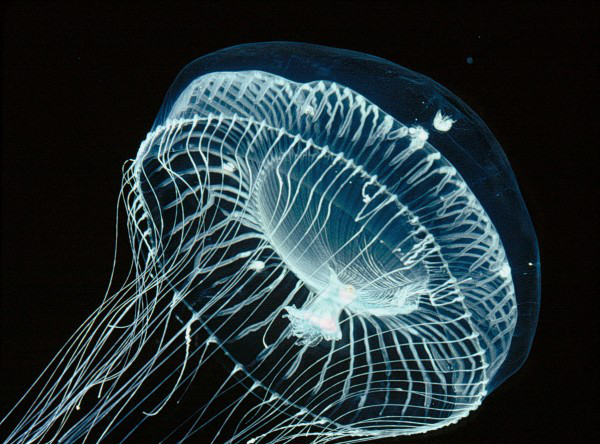
\includegraphics[width=0.9\linewidth]{medusasenzarif}
\caption{Aequorea victoria}
\end{figure}

\column{0.5\textwidth}
This formula has a very intuitive interpretation as the so-called stationary phase approximation: suppose that the light emitted from the A.v. travels in spherical waves.

\end{columns}
\end{frame}

%------------------------------------------------

\begin{frame}
\frametitle{The stationary phase approximation (II)}
\begin{columns}[c]
\column{0.5\textwidth}
\begin{figure}
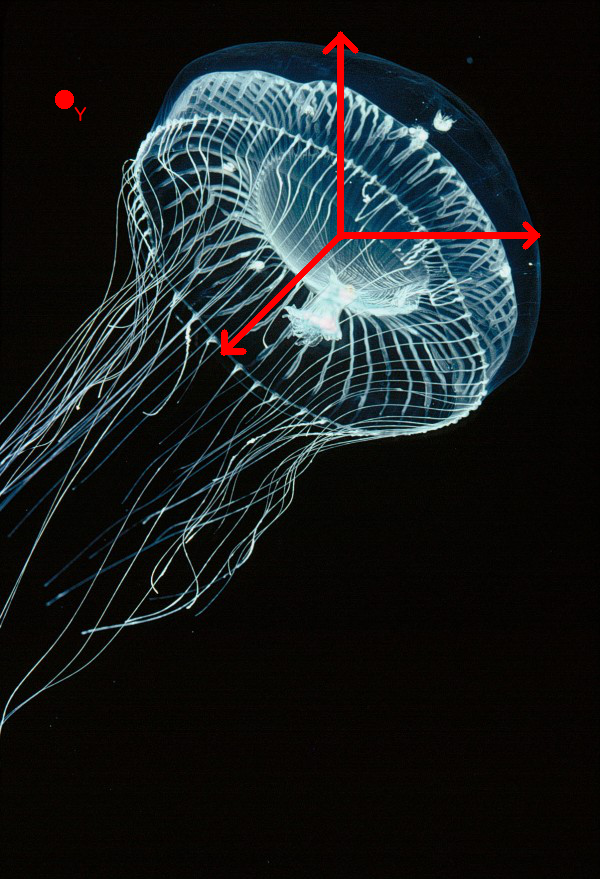
\includegraphics[width=0.75\linewidth]{medusatot}
\caption{Aequorea victoria}
\end{figure}

\column{0.5\textwidth}
The intensity in $y$ can be computed as
\[
\begin{split}
I(y)&=\int_{\mathbb R^3}\nu(x)\frac{e^{ik||x-y||}}{||x-y||}d^3x\\
&=\int_{\mathbb R^3}a(x)e^{ik\phi(x)}d^3x
\end{split}
\]
where $\nu(x)$ is the density of the A.v.\newline
$k$ is "large" $\Rightarrow$ Main contributions in the stationary points of $\phi$.
\end{columns}
\end{frame}

%------------------------------------------------

\subsection{Generalized flag manifolds}
\begin{frame}
\frametitle{Fixed points}
\begin{definition}{}
Generalized flag manifolds can be equivalently defined as:
\begin{itemize}
\item
Quotients $G/C(S)$, where $C(S)$ is the centralizer of a torus $S$ in $G$;
\item
Orbits of the adjoint action of $G$ on $\frak g$.
\end{itemize}
\end{definition}
Let us take the first point of view. We have the following
\begin{theorem}
The fixed point action of a maximal torus $T\subset G$ on $G/C(S)$ has finitely many fixed points, corresponding to representatives of $W(G)/W(C(S))$.
\end{theorem}
\end{frame}

%------------------------------------------------

\begin{frame}
\frametitle{The moment map}
Suppose that the group $G$ is semisimple. This has two consequences:
\begin{itemize}
\item Given a symplectic action of $G$, there exists a unique moment map;
\item The adjoint representation is isomorphic to the coadjoint representation.
\end{itemize}
One proves that there exists a canonical symplectic structure, with moment map of the $T$-action
\[
\varphi:M\hookrightarrow\frak g^*\simeq\frak t^*
\]
\end{frame}

%------------------------------------------------

\begin{frame}
\frametitle{Conclusions}
\begin{itemize}
\item Localization is a powerful machinery, which condensates information from the whole space to a set of points;
\item This advantages are however only apparent, unless we can elaborate the data on points;
\item This is the case for GFM. We saw how to derive the position of points and the moment map for the canonical symplectic form;
\item The product of weights $\Pi_j\alpha^i_j$ carries local information about the moment map, as can be seen from the stationary phase approximation: not easy to compute.
\end{itemize}
\end{frame}

%----------------------------------------------------------------------------------------

\end{document} 